\chapter{数值模拟示例}\label{chap:appendix-d}

\begin{note}[一般考虑]\label{note:appendix-d-1}
如何定义恰当的测试算例,对评估数值格式十分重要.测试问题大致分为以下几类.
\begin{itemize}
  \item \textbf{给定解析解的学术测试算例.}这类算例用解析函数给出速度场 $\bm u$ 和压力 $p$,并相应选取右端项、边界条件和初始条件,使所研究方程的强形式成立.这类算例可用于支持收敛性估计,通常与实际问题没有直接联系.定义算例时,必须确保速度场无散;此外,根据边界条件的类型(见第\hyperref[sec:initial-boundary]{2.4}节),还须满足压力积分平均值为零,或 Dirichlet 边界数据的积分满足相容条件\hyperref[eq:dirichlet-flux-compatibility]{(2.33)}.
  \item \textbf{具有真实流动特征的学术测试算例.}这类算例一方面包含实际流动问题的一些重要特征,另一方面又作了若干简化,以便实现算例并评估结果.通常不存在解析解.感兴趣的量的参考值由空间和时间上极细网格的数值模拟得到.
  \item \textbf{实际问题.}数值方法应能良好地处理这类问题.然而,实际问题中的数据常不完整,例如通常没有时空分辨的边界条件.用于比较的参考值往往来自测量,通常是空间或时间平均值,而且测量误差不可避免.因此,评估实际流动问题中的数值方法需要特别谨慎,也需要专门技术.由于数据不完整,任何方法一般都不可能给出与真实流动完全一致的结果;必须以恰当的方式评估差异.
\end{itemize}
本附录列出本书数值算例中使用的一些问题,其中大多数是文献中的标准测试问题.所有模拟均使用 MooNMD 程序包完成,见\textcite{JohnMatthies2004}.
\end{note}

\begin{note}[流动作用于物体的力]\label{note:appendix-d-2}
考虑流场中的物体,其边界记为 $\Gamma_{\mathrm{body}}$.流体沿单位方向 $\bm w$ 作用于物体的力为
\[
\begin{aligned}
 F_{\bm w}
 &=-\int_{\Gamma_{\mathrm{body}}}(\symbf{\sigma}\bm n)\cdot\bm w\,\mathrm ds\\
 &=-\int_{\Gamma_{\mathrm{body}}}
   \bigl((2\mu D(\bm v)-P I)\bm n\bigr)\cdot\bm w\,\mathrm ds
   \quad[\mathrm N].
\end{aligned}
\]
这里 $\bm n$ 是相对于流动区域 $\Omega$ 指向外侧的单位法向量,应力张量见式\hyperref[eq:dimensionless-stress-tensor]{(2.18)}.因此,该力是法向应力的负值在方向 $\bm w$ 上的投影.由无量纲变量关系\hyperref[eq:dimensionless-parameters]{(2.23)},可得
\begin{equation}\label{eq:appendix-d-1}
\begin{aligned}
F_{\bm w}
 &=-L^{d-1}\int_{\Gamma_{\mathrm{body}}}
 \left(\frac{2\mu U}{L}D(\bm u)-\rho U^2pI\right)\bm n\cdot\bm w\,\mathrm ds\\
 &=-\rho U^2L^{d-1}\int_{\Gamma_{\mathrm{body}}}
 \left(\frac{2\mu}{\rho UL}D(\bm u)-pI\right)\bm n\cdot\bm w\,\mathrm ds\\
 &=-\rho U^2L^{d-1}\int_{\Gamma_{\mathrm{body}}}
 \bigl((2\nu D(\bm u)-pI)\bm n\bigr)\cdot\bm w\,\mathrm ds ,
\end{aligned}
\end{equation}
其中无量纲黏度为 $\nu=\mu/(\rho UL)=\mathrm{Re}^{-1}$.第一行中的 $1/L$ 来自空间导数的变换,因子 $L^{d-1}$ 来自积分的变换.

公式\hyperref[eq:appendix-d-1]{(D.1)} 可自然地写入 Navier--Stokes 方程的变分形式.假设物体边界没有与流动区域其余部分相连,即 $\Gamma_{\mathrm{body}}\cap\partial\Omega=\varnothing$.可将 $\bm w$ 延拓为 $\Omega$ 上的函数,使其属于 $H^1(\Omega)^d$,并在 $\partial\Omega\setminus\Gamma_{\mathrm{body}}$ 上为零.用 $\bm w$ 检验动量方程\hyperref[eq:dimensionless-ns-standard]{(2.25)} 并分部积分,得到
\[
\begin{aligned}
 (\partial_t\bm u,\bm w)
 +(2\nu D(\bm u),D(\bm w))
 +((\bm u\cdot\nabla)\bm u,\bm w)\\
 &-(\nabla\cdot\bm w,p)\\
 &-\langle\bm f,\bm w\rangle_{(H^1(\Omega))',H^1(\Omega)}\\
 &=\int_{\Gamma_{\mathrm{body}}}\\
 &\qquad\bigl((2\nu D(\bm u)-pI)\bm n\bigr)\\
 &\qquad\qquad\cdot\bm w\,\mathrm ds .
\end{aligned}
\]
于是
\begin{equation}\label{eq:appendix-d-2}
\begin{aligned}
F_{\bm w}=-\rho U^2L^{d-1}\bigl[
 &(\partial_t\bm u,\bm w)
 +(2\nu D(\bm u),D(\bm w))
 +((\bm u\cdot\nabla)\bm u,\bm w)\\
 &-(\nabla\cdot\bm w,p)
 -\langle\bm f,\bm w\rangle_{(H^1(\Omega))',H^1(\Omega)}
\bigr].
\end{aligned}
\end{equation}
稳态问题中的时间导数项为零.黏性项和对流项均有不同写法,见式\hyperref[eq:stokes-deformation-tensor-form]{(4.5)}及第\hyperref[subsec:steady-ns-nonlinear-term]{6.1.2}节.在连续情形中,由于 $\bm u$ 弱无散,这些写法等价,因而所得力公式也等价.但在有限元方法中,这种等价性通常不再成立;黏性项或对流项选用不同形式,会使离散力的近似值不同.据我们所知,目前尚无研究量化这种差异.

实际计算中,即使物体与流动区域的其余边界相连,也常使用公式\hyperref[eq:appendix-d-2]{(D.2)}计算 $F_{\bm w}$.例如,圆柱绕流见\textcite{John2002}及例题\hyperref[ex:appendix-d-6]{D.6},壁面立方体绕流见\textcite{Hoffman2005}、\textcite{HoffmanJohnson2006}及例题\hyperref[ex:appendix-d-14]{D.14}.

应用中一个重要的量是沿主流方向的力,即阻力.以此定义无量纲阻力系数
\begin{equation}\label{eq:appendix-d-3}
 c_{\mathrm{drag}}=\frac{2F_{\mathrm{drag}}}{\rho A V^2},
\end{equation}
其中 $V$ 表示障碍物相对于流体的速度尺度,$A$ 为参考面积.$\rho V^2/2$ 称为动压.由式\hyperref[eq:appendix-d-1]{(D.1)}可得
\begin{equation}\label{eq:appendix-d-4}
c_{\mathrm{drag}}
=-\frac{2U^2L^{d-1}}{AV^2}
\int_{\Gamma_{\mathrm{body}}}
\bigl((2\nu D(\bm u)-pI)\bm n\bigr)\cdot\bm w_{\mathrm{drag}}\,\mathrm ds,
\end{equation}
由式\hyperref[eq:appendix-d-2]{(D.2)}则有
\begin{equation}\label{eq:appendix-d-5}
\begin{aligned}
c_{\mathrm{drag}}=-\frac{2U^2L^{d-1}}{AV^2}\Bigl[&
(\partial_t\bm u,\bm w_{\mathrm{drag}})
+(2\nu D(\bm u),D(\bm w_{\mathrm{drag}}))\\
&+((\bm u\cdot\nabla)\bm u,\bm w_{\mathrm{drag}})
-(\nabla\cdot\bm w_{\mathrm{drag}},p)\\
&-\langle\bm f,\bm w_{\mathrm{drag}}\rangle_{(H^1(\Omega))',H^1(\Omega)}
\Bigr].
\end{aligned}
\end{equation}

同样重要的是垂直于主流方向的力,即升力.若主流方向为
$\bm w_{\mathrm{drag}}=(w_1,w_2,0)^\mathsf T$,则取其正交方向
$\bm w_{\mathrm{lift}}=(-w_2,w_1,0)^\mathsf T$.升力系数定义为
\begin{equation}\label{eq:appendix-d-6}
 c_{\mathrm{lift}}=\frac{2F_{\mathrm{lift}}}{\rho A V^2}.
\end{equation}
相应地,
\begin{equation}\label{eq:appendix-d-7}
c_{\mathrm{lift}}
=-\frac{2U^2L^{d-1}}{AV^2}
\int_{\Gamma_{\mathrm{body}}}
\bigl((2\nu D(\bm u)-pI)\bm n\bigr)\cdot\bm w_{\mathrm{lift}}\,\mathrm ds,
\end{equation}
\begin{equation}\label{eq:appendix-d-8}
\begin{aligned}
c_{\mathrm{lift}}=-\frac{2U^2L^{d-1}}{AV^2}\bigl[
 &(\partial_t\bm u,\bm w_{\mathrm{lift}})
 +(2\nu D(\bm u),D(\bm w_{\mathrm{lift}}))
 +((\bm u\cdot\nabla)\bm u,\bm w_{\mathrm{lift}})\\
 &-(\nabla\cdot\bm w_{\mathrm{lift}},p)
 -\langle\bm f,\bm w_{\mathrm{lift}}\rangle_{(H^1(\Omega))',H^1(\Omega)}
\bigr],
\end{aligned}
\end{equation}
其中式\hyperref[eq:appendix-d-7]{(D.7)} 来自公式\hyperref[eq:appendix-d-1]{(D.1)},式\hyperref[eq:appendix-d-8]{(D.8)} 来自公式\hyperref[eq:appendix-d-2]{(D.2)}.文献中还可找到阻力和升力的其他计算公式.例如,\textcite{SchaeferTurek1996} 针对特殊情形 $\bm w_{\mathrm{drag}}=(1,0,0)^\mathsf T$ 且 $\partial_z u_3|_{\Gamma_{\mathrm{body}}}=0$ 给出了一组公式.
\end{note}

\section{稳态流动算例}\label{sec:appendix-d-1}

\begin{example}[单位正方形上给定解、齐次 Dirichlet 边界条件的二维稳态算例]\label{ex:appendix-d-3}
考虑 $\Omega=(0,1)^2$,并定义流函数
\[
 \psi=1000x^2(1-x)^4y^3(1-y)^2.
\]
速度场取为
\begin{equation}\label{eq:appendix-d-9}
\bm u=
\begin{pmatrix}u_1\\u_2\end{pmatrix}
=\begin{pmatrix}\partial_y\psi\\-\partial_x\psi\end{pmatrix}
=1000\begin{pmatrix}
x^2(1-x)^4y^2(1-y)(3-5y)\\
-2x(1-x)^3(1-3x)y^3(1-y)^2
\end{pmatrix}.
\end{equation}
由 Schwarz 定理,
\[
\nabla\cdot\bm u
=\partial_xu_1+\partial_yu_2
=\partial_{xy}\psi-\partial_{yx}\psi=0.
\]
在整个边界 $\partial\Omega$ 上施加 Dirichlet 条件.由于边界上 $\bm u=0$,相容条件\hyperref[eq:dirichlet-flux-compatibility]{(2.33)}成立.此处边界条件意味着压力应属于 $L_0^2(\Omega)$;这是唯一实质性要求.该算例选取如下压力:
\[
 p=\pi^2\bigl(xy^3\cos(2\pi x^2y)-x^2y\sin(2\pi xy)\bigr)+\frac18.
\]
图\hyperref[fig:appendix-d-1]{D.1}展示了流函数、速度和压力;速度场主要由一个大涡旋构成.由于该算例采用齐次 Dirichlet 条件,它符合有限元数值分析中许多结果的适用框架.
\begin{elegantfigure}[0.92\linewidth]
 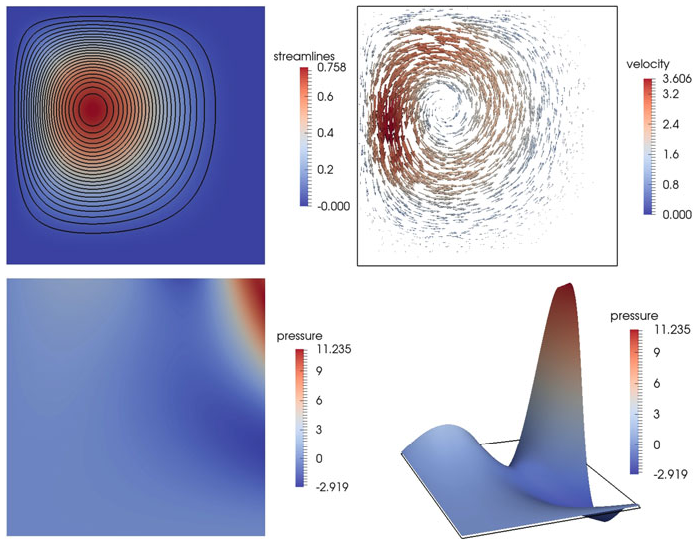
\includegraphics[width=\linewidth]{figures/Appendix_D/Fig_D_01__PDFp758__Bookp753.pdf}
 \captionof{figure}{例题 D.3:流函数(左上)、速度(右上)和压力(下);这些图由数值模拟结果绘制.}\label{fig:appendix-d-1}
\end{elegantfigure}
\end{example}

\begin{example}[二维驱动方腔问题]\label{ex:appendix-d-4}
二维驱动方腔问题是二维稳态流动中最常用的测试算例.区域为 $\Omega=(0,1)^2$,体力为零,即 Navier--Stokes 方程\hyperref[eq:steady-ns-strong]{(6.1)}中的右端项 $\bm f=0$.经典驱动方腔问题的边界条件通常写为
\begin{equation}\label{eq:appendix-d-10}
\bm u=\begin{pmatrix}0\\0\end{pmatrix}
\quad\text{当 }x=0,\ x=1\text{ 或 }y=0,\qquad
\bm u=\begin{pmatrix}1\\0\end{pmatrix}
\quad\text{当 }y=1.
\end{equation}
各算例由雷诺数 $\mathrm{Re}=\nu^{-1}$ 确定.

边界条件\hyperref[eq:appendix-d-10]{(D.10)}在方腔上角处有跳跃.若采用 Taylor--Hood 等有限元空间对,就必须指定速度在两个角点处的值.只有部分文献明确给出这种取值,例如\textcite{Olshanskii2002} 取
$\bm u(0,1)=\bm u(1,1)=(1,0)^\mathsf T$.无论角点处具体取何值,Dirichlet 边界数据都不属于 $H^{1/2}(\partial\Omega)$;由 $s=1$ 时的迹定理\hyperref[thm:appendix-a-34]{A.34},速度不可能属于 $H^1(\Omega)$.因此,经典驱动方腔问题不符合第\hyperref[chap:steady-navier-stokes]{6}章的理论框架.严格地说,该解的正则性不足以使用协调有限元方法.

经典驱动方腔问题的参考解通常取自\textcite{Ghia1982},其中给出了
$\mathrm{Re}\in\{100,400,1000,3200,5000,7500,10000\}$ 时的流线、截线上的解剖面和涡旋中心位置.然而,\textcite{Cazemier1998}、\textcite{Tiesinga2002}、\textcite{BruneauSaad2006} 等研究表明,经典顶盖驱动方腔的稳态解在 $\mathrm{Re}\approx8000$ 时失稳;当 $\mathrm{Re}=10000$ 时存在稳定的周期解.因此,若数值方法在 $\mathrm{Re}=10000$ 时得到稳定稳态解,就必须引入额外数值黏性.事实上,\textcite{Ghia1982} 使用有限差分格式,并采用了某种迎风型稳定化.

为消除上角点处的奇异性,文献提出了正则化驱动方腔问题,例如见\textcite[第 125 页]{Elman2014}.定义此类问题时,必须确保边界上也满足 $\nabla\cdot\bm u=0$,且角点处的散度完全由给定边界条件确定.\textcite{deFrutos2016c} 提出的一种满足这些要求的正则化问题采用如下边界条件:
\begin{equation}\label{eq:appendix-d-11}
\begin{aligned}
\bm u(x,1)&=\begin{pmatrix}u_1(x)\\0\end{pmatrix},\\
u_1(x)&=\begin{cases}
1-\tfrac14\bigl(1-\cos(\pi(x_1-x)/x_1)\bigr)^2,&x\in[0,x_1],\\[1mm]
1,&x\in(x_1,1-x_1),\\[1mm]
1-\tfrac14\bigl(1-\cos(\pi(x-(1-x_1))/x_1)\bigr)^2,&x\in[1-x_1,1].
\end{cases}
\end{aligned}
\end{equation}
本书所示模拟均取 $x_1=0.1$.图\hyperref[fig:appendix-d-2]{D.2}展示了
$\mathrm{Re}=1$ 和 $\mathrm{Re}=3200$ 时的解.低雷诺数时有一个靠近上边界的大涡旋,压力在两个上角处均出现较高峰值.$\mathrm{Re}=3200$ 时,速度场包含一个位于方腔中心附近的大涡旋、两个下角处的反向小涡旋,以及左边界上部的一个反向小涡旋;压力在右上角达到正峰值.
\begin{elegantfigure}[0.94\linewidth]
 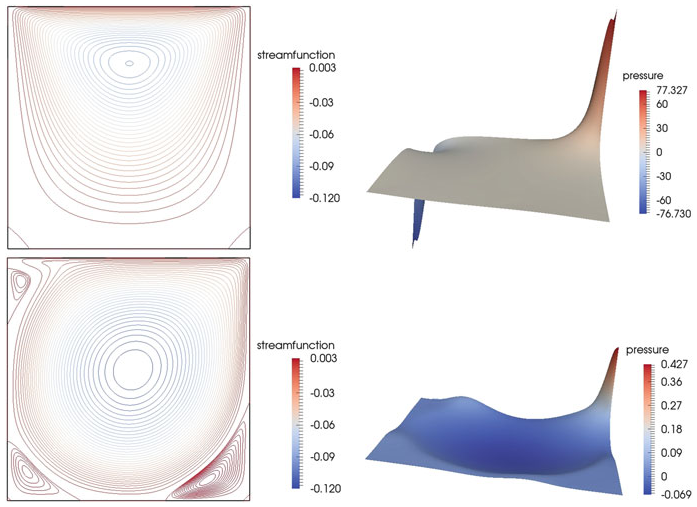
\includegraphics[width=\linewidth]{figures/Appendix_D/Fig_D_02__PDFp760__Bookp755.pdf}
 \captionof{figure}{例题 D.4:满足边界条件\hyperref[eq:appendix-d-11]{(D.11)}的正则化驱动方腔问题.$\mathrm{Re}=1$(上)和 $\mathrm{Re}=3200$(下)的流函数与压力.}\label{fig:appendix-d-2}
\end{elegantfigure}
\end{example}
